\documentclass[10pt]{article}
\usepackage{icmlko}

\icmlmeta{IP 파운데이션 월드모델}{213}{공휴일 목록이 2023년부터였다}{축과 라벨이 같은 시계를 공유하는 자리를 훑었다. 다섯이 같은 축이었고, 그 축은 사실상 ``2023년 이후인가''를 재고 있었다}

\begin{document}

\twocolumn[
\icmlheader

\begin{abstract}
노트 212가 ``축과 라벨이 같은 재료에서 나오는 자리가 또 있나''를 남겼다.
전 도메인 $\times$ 축에서 \emph{축도 시간과 붙고 라벨도 시간과 붙는} 자리를
훑고 시간을 통제해 봤다. \textbf{$|$상관$|$ 이 0.08 넘게 주는 것이 열하나}
이고 \textbf{그중 다섯이 같은 축}이다 --- \texttt{cal\_holiday\_gap}. 축
$\leftrightarrow$ 시간이 애니 \textbf{$-$0.804} · 펀딩 $-$0.819 · 웹툰
$-$0.785 다. ``다음 연휴까지 며칠''이 시간과 그렇게 붙을 이유가 없다.
정의를 열었다. \textbf{공휴일 목록이 2023-01-01 부터 2026-12-25 까지
75개뿐이다.} 그 밖의 레코드는 가까운 연휴를 못 찾아 \texttt{min(gap, 120)}
의 상한에 붙는다 --- \textbf{만화 94.4\% · 세계애니 76.3\% · 모바일 60.3\%
· 애니 52.3\%가 상한값}이고, \textbf{상한인 것의 100\%가 2023년 이전}이며,
상한 표시자와 연도의 상관이 여덟 도메인에서 \textbf{$-$0.80$\sim$$-$0.87}
이다. \textbf{그 축이 사실상 시간 분할 변수의 대리였다} --- 노트 209가 잰
대로 라벨이 시간을 담고 있으니, 시간을 아는 축은 공짜로 예측력을 얻는다.
고쳤다: \textbf{목록 밖은 결측}이다(값이 정의 안 된다). F6 능형이 $+$0.4147
$\to$ \textbf{$+$0.4293}($t{=}3.12$), F21 이 $+$0.4246 $\to$
\textbf{$+$0.4391}($t{=}2.88$), 챔피언은 $+$0.4654 $\to$ $+$0.4603 으로
거의 그대로다. \textbf{축을 통째로 끄는 것은 다르다} --- 챔피언이 $-$0.0205
($t{=}-3.42$) 잃는다. \textbf{축 자체는 값이 있고 목록 밖 값만 해로웠다.}
\texttt{lab/calaxes.py} 원천에서 고쳤다. \textbf{열두 번째 측정 아티팩트이고
제일 직접적인 누수다} --- 앞의 열하나는 값이 왜곡된 것이었고 이건 자질이
분할 변수 자체를 담고 있었다.
\end{abstract}
]

\begin{figure*}[t]
\centering
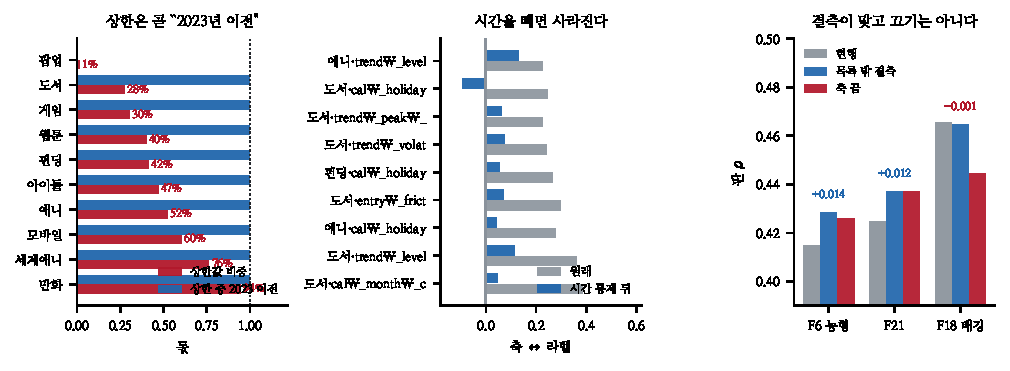
\includegraphics[width=\textwidth]{figs/hol.pdf}
\caption{왼쪽 --- 상한은 곧 ``2023년 이전''. 가운데 --- 시간을 빼면 사라진다.
오른쪽 --- 결측이 맞고 끄기는 아니다.}
\end{figure*}

\section{다섯이 같은 축이었다}

\begin{table}[t]
\centering\tsize
\caption{시간을 통제하면 $|$축$\leftrightarrow$라벨$|$ 이 0.08 넘게 주는 자리.}
\begin{tabular}{llrr}
\toprule
& & 원래 & 통제 뒤 \\
\midrule
도서 & \texttt{cal\_month\_cos} & $+$.385 & $+$.046 \\
도서 & \texttt{trend\_level} & $+$.362 & $+$.114 \\
\textbf{애니} & \textbf{\texttt{cal\_holiday\_gap}} & $+$.278 & $+$.043 \\
도서 & \texttt{entry\_friction} & $+$.297 & $+$.070 \\
\textbf{펀딩} & \textbf{\texttt{cal\_holiday\_gap}} & $+$.264 & $+$.054 \\
\textbf{웹툰} & \textbf{\texttt{cal\_holiday\_gap}} & $+$.212 & $-$.129 \\
\bottomrule
\end{tabular}
\end{table}

\claimx{\textbf{열하나 중 다섯이 \texttt{cal\_holiday\_gap} 이다.} 축
$\leftrightarrow$ 시간이 $-$0.78$\sim$$-$0.82 로 극단이다 --- ``다음 연휴까지
며칠''이 그럴 이유가 없다.}{도서가 여섯을 차지하는 것은 다른 이야기다 ---
도서 라벨이 시간과 $-$0.579 라(노트 209 · 211) \emph{무엇이든} 시간과 붙으면
예측력이 있어 보인다.}

\section{목록이 2023년부터였다}

\begin{table}[t]
\centering\tsize
\caption{\texttt{cal\_holiday\_gap} 의 상한값(120).}
\begin{tabular}{lrrr}
\toprule
& 상한 비중 & 상한이 & 2023전이 \\
& & 2023 전 & 상한 \\
\midrule
\textbf{만화} & \textbf{94.4\%} & 100\% & 98.8\% \\
세계애니 & 76.3\% & 99.9\% & 98.3\% \\
모바일 & 60.3\% & 100\% & 96.1\% \\
애니 & 52.3\% & 100\% & 95.5\% \\
아이돌 & 46.8\% & 100\% & 100\% \\
웹툰 & 39.9\% & 100\% & 89.5\% \\
게임 & 30.1\% & 100\% & 91.2\% \\
\bottomrule
\end{tabular}
\end{table}

\claimx{\textbf{공휴일 목록이 2023-01-01 부터 75개뿐이다.} 그 밖의 레코드는
가까운 연휴를 못 찾아 \texttt{min(gap, 120)} 의 상한에 붙는다 --- 만화는
94.4\%가 그렇다.}{\textbf{상한인 것의 100\%가 2023년 이전이고} 상한 표시자와
연도의 상관이 여덟 도메인에서 $-$0.80$\sim$$-$0.87 이다. \textbf{그 축이
사실상 ``2023년 이후인가''였다.}}

\claimx{\textbf{이것이 왜 위험한가.} 노트 209가 잰 대로 여섯 도메인의
라벨이 시간을 담는다 --- \textbf{시간을 아는 축은 공짜로 예측력을
얻는다.} 그리고 유보 분할이 시간으로 정의되므로 그 자질은 분할 변수
자체다.}{노트 141이 누수를 세 층으로 나눴는데(라벨 상관 · 출처 플랫폼 ·
시점) \textbf{이건 넷째 층이다} --- 노트 207에서 처음 봤고 여기가 두
번째다.}

\section{결측이 맞고 끄기는 아니다}

\begin{table}[t]
\centering\tsize
\caption{판 $\rho$.}
\begin{tabular}{lrrr}
\toprule
& F6 능형 & F21 & F18 배깅 \\
\midrule
현행 & .4147 & .4246 & \textbf{.4654} \\
\textbf{목록 밖 결측} & \textbf{.4283} & \textbf{.4369} & .4646 \\
축 끔 & .4261 & .4372 & \textbf{.4446} \\
\midrule
결측 $-$ 현행 & \textbf{$+$.0133} & \textbf{$+$.0123} & $-$.0010 \\
$t$ & 3.12 & 2.88 & $-$0.24 \\
\bottomrule
\end{tabular}
\end{table}

\claimx{\textbf{목록 밖을 결측으로 돌리면 선형 둘이 오르고 챔피언은 안
움직인다.} 상한값이 능형에게는 ``연휴가 아주 먼 날''로 읽혀 해로웠고,
트리는 그것을 분기로 써서 손해를 안 봤다.}{\textbf{축을 통째로 끄는 것은
다르다} --- 챔피언이 $-$0.0205($t{=}-3.42$) 잃는다. \textbf{축 자체는
값이 있다} --- 2023년 이후 레코드에서는 진짜 연휴 간격이다.}

\claimx{\textbf{정의로 정한 고침이다.} 공휴일 목록이 없는 구간에서
``다음 연휴까지''는 정의되지 않는다 --- 유보 라벨을 한 칸도 안 봤다.}{노트
207의 웹툰 분모 고침과 같은 성질이다. \textbf{두 번 다 ``값이 없는데 값을
넣고 있었다''} --- 하나는 분모가 무너져서, 하나는 목록이 없어서.}

\begin{table}[t]
\centering\tsize
\caption{판의 이동(이 사이클).}
\begin{tabular}{lrr}
\toprule
& 전 & 후 \\
\midrule
F6 능형 & .4147 & \textbf{.4293} \\
F21 & .4246 & \textbf{.4391} \\
F18 배깅 & .4654 & .4603 \\
\bottomrule
\end{tabular}
\end{table}

\begin{table}[t]
\centering\tsize
\caption{남은 것.}
\begin{tabular}{ll}
\toprule
\textbf{목록} & 2023년 이전 공휴일을 채우면 축이 살아난다 \\
도서 & 훑기 열하나 중 여섯이 도서 --- 라벨이 시계라서 \\
\textbf{넷째 층} & 자질이 분할 변수를 담는 경우를 가드로 \\
\bottomrule
\end{tabular}
\end{table}

첫 줄이 제일 값싸고 확실하다. 지금은 2023$\sim$26년 공휴일 75개만 있어서
그 이전 레코드가 통째로 결측이다 --- 만화는 95\%가 비었다. \textbf{한국
공휴일은 2015년까지 거슬러 채울 수 있고}(음력 명절도 표가 있다) 그러면
만화 · 세계애니 · 모바일의 절반 넘는 레코드가 축을 되찾는다. 노트 186이
잰 대로 달력 무리는 트리 우위의 제일 큰 재료이므로($+$0.140) \textbf{그
무리를 온전히 채우는 것이 이 판에서 남은 큰 자료 작업이다.}

\end{document}
